% Document class & environment definition -----------------------------------------------
\documentclass[10pt]{report}

\usepackage[utf8]{inputenc}

\usepackage[english]{babel}

\usepackage[T1]{fontenc}

\usepackage{setspace}

\usepackage{amsfonts}

\usepackage{harmony}

\usepackage{graphicx}
\graphicspath{ {./images/} }

\usepackage{geometry}
\geometry{a4paper, top=2cm, bottom=2cm, left=2cm, right=2cm}

\usepackage{amsmath}
\numberwithin{section}{chapter}
\numberwithin{equation}{section}
\numberwithin{figure}{chapter}

\usepackage[a-2b,mathxmp]{pdfx}
\usepackage[pdfa]{hyperref}

\usepackage{xcolor}
\usepackage{color}

\definecolor{codegreen}{rgb}{0,0.6,0}
\definecolor{codegray}{rgb}{0.5,0.5,0.5}
\definecolor{codepurple}{rgb}{0.58,0,0.82}
\definecolor{backcolour}{rgb}{0.95,0.95,0.92}


\usepackage{listings}
\lstdefinestyle{mystyle}
{
	backgroundcolor=\color{backcolour},   
	commentstyle=\color{codegreen},
	keywordstyle=\color{magenta},
	numberstyle=\tiny\color{codegray},
	stringstyle=\color{codepurple},
	basicstyle=\ttfamily\footnotesize,
	breakatwhitespace=false,         
	breaklines=true,                 
	captionpos=b,                    
	keepspaces=true,                 
	numbers=left,                    
	numbersep=5pt,                  
	showspaces=false,                
	showstringspaces=false,
	showtabs=false,                  
	tabsize=2
}
\lstset{style=mystyle}


%\usepackage{fancyhdr}
%\pagestyle{fancy}
%\lhead{}
%\chead{}
%\rhead{}
%\lfoot{Consorzio RFX - Ricerca, Formaxzione, Innovazione}
%\cfoot{}
%\rfoot{\thepage}

\usepackage{subcaption}


% Commands ------------------------------------------------------------------------------
\newcommand{\Cels}{^{\circ}C}
\newcommand{\half}{\frac{1}{2}}
\renewcommand\thesection{\arabic{section}}
%\renewcommand{\headrulewidth}{0.5pt}
%\renewcommand{\footrulewidth}{0.5pt}


\begin{document}
	
	\begin{titlepage}
		\begin{center}
			
\includegraphics[width=0.5\textwidth]{images/rfx_logo.png}
			\vspace{1.5cm}
			\Huge 
			\doublespacing 
			\bfseries 
			\begin{spacing}{1}
				\textsc{KRIA KR260 Robotics Starter Kit: the first steps}
			\end{spacing}
			\vfill
			\small
			Authors: Bevilacqua Mattia, Gabriele Manduchi\\
			Date : \today 
		\end{center}
	\end{titlepage}
	
	\clearpage
	\null
	\thispagestyle{empty}
	\clearpage
	
	\tableofcontents
	
	\clearpage
	\null
	\thispagestyle{empty}
	\clearpage
	
	\chapter{Introduction}
Approaching the world of Filed Programmable Gate Arrays (FPGAs) programming, specially when combined with micro processor units (uPs) to form the so-called System on Modules (SoMs), is far from being a straight procedure and one can easily get stuck trying to solve problems that can be avoided with a bit of experience. The aim of this guide is thus to share the experience and knowledge gained while working on such devices and give some standard procedure on how to approach and solve the problems that may be encountered. Some useful links are reported in the list below:
\begin{itemize}
	\item \textbf{Petalinux Build Host packages}:  \url{https://adaptivesupport.amd.com/s/article/73296?language=en\_US} 
	
	\item \textbf{AMD download page}:  \url{https://www.xilinx.com/support/download/index.html/content/xilinx/en/downloadNav/embedded-design-tools/archive.html}
\end{itemize} 
This guide presents an overview of four projects. Chapter 2 introduces the first project, which involves creating a classic blinking LED using only FPGA programming. Chapter 3 revisits  the same project but incorporates a custom operating system (OS) configuration. While this addition is not particularly necessary for the blinking LED, it establishes a foundation for the next projects. Chapter 4 focuses on implementing two First-In, First-Out (FIFO) memories to enhance communication capabilities. Finally, chapter 5 will implement the same R/W operations using the Direct Memory Access (DMA).  


\section{Requirements}
To program FPGA devices, software tools are usually provided by the manufacturer. Being hybrid devices, it is necessary to set up a custom environment through which the required design steps can be carried out and the final result translated into a language understandable by the device. The board used in this guide is the Xilinx Kria KR260 Robotics Starter Kit, which needs a toolchain in order to be fully exploited. Fundamental part of the toolchain are:
\begin{itemize}
	\item Vivado (v2024.1).
	
	\item Petalinux SDK (v2022.2).
	
	\item Linux based OS (for this guide CenOS stream 9 has been used).
\end{itemize}
Newest software releases might not be compatible with the procedure(s) listed and/or with the files used to support the processes. It is recommended to check resources availability and compatibility before the installation of both Vivado and Petalinux SDK.

\section{Environment configuration}
The installation of Vivado is a straightforward process with no complex steps, requiring no special attention. Downloading it from the Xilinx download page should be an easy step, thus it is not reported below. On the other hand, more attention is given to the configuration of Petalinux SDK. Before the actual installation, there are few steps needed to configure the foundations:
\begin{enumerate}
	\item Enable the 32-bit support. The 32-bit architecture is required on the host machine because some PetaLinux tools and dependencies rely on 32-bit libraries. From the terminal window type
	\begin{lstlisting}[language=bash]
		sudo yum install glibc.i686 libstdc++.i686 ncurses-libs.i686 zlib.i686	\end{lstlisting}
	In the case the host machine is running on Ubuntu, the command to install the required architecture is
	\begin{lstlisting}[language=bash]
		sudo dpkg --add-architecture i386
		dpkg --print-foreign-architectures	\end{lstlisting}
	
	\item Petalinux Build Host packages. These files are required to install all the secondary packages necessary for running PetaLinux commands on the system. First, create a directory where the PetaLinux SDK will be installed. From the  \href{https://adaptivesupport.amd.com/s/article/73296?language=en_US}{Petalinux Build Host packages} page download the file named \textit{plnx-env-setup.sh} and save it into the folder just created. To start the installation of all the packages type
	\begin{lstlisting}[language=bash]
		chmod +x <installer_file_name>
		sudo ./<file_name>	\end{lstlisting}
\end{enumerate}
Once it is completed, all the packages should have been installed and the system should be ready for the Petalinux SDK installation. From the \href{https://www.xilinx.com/support/download/index.html/content/xilinx/en/downloadNav/embedded-design-tools/archive.html}{AMD download page}, download the needed version and move it to the installation folder. From this page also download the .BPS file relative to the board to be used. This latter file has to be moved into the folder in which the Petalinux project are saved. By typing
	\begin{lstlisting}[language=bash]
	chmod +x <installer_file_name>
	sudo ./<file_name>	
\end{lstlisting}
the installation should begin. By following the instruction, the installation process
should proceed without any inconvenience, even though it might take a while. Finally, to set the Petalinux environment into the directory in which it is installed, type
\begin{lstlisting}[language=bash]
	source settings.sh
\end{lstlisting}
Note that this latter step is needed each time a new project is created.
	\chapter{Bare Metal Programming}
Bare-Metal Programming (BMP) is a common approach in embedded systems where software runs directly on hardware without requiring an operating system. This method provides direct control over hardware resources, ensuring low latency and high performance. Additionally, debugging techniques are explored to analyze and optimize the code execution.

\section{Vivado}
Vivado is a software developed by AMD, oriented to programming FPGAs, which supports various board and modules. The example project that will be discussed within this chapter is meant only to give an introduction to the Vivado-FPGA programming world, which is way more vast and deeper.
\begin{figure}[h!t!]
	\centering
	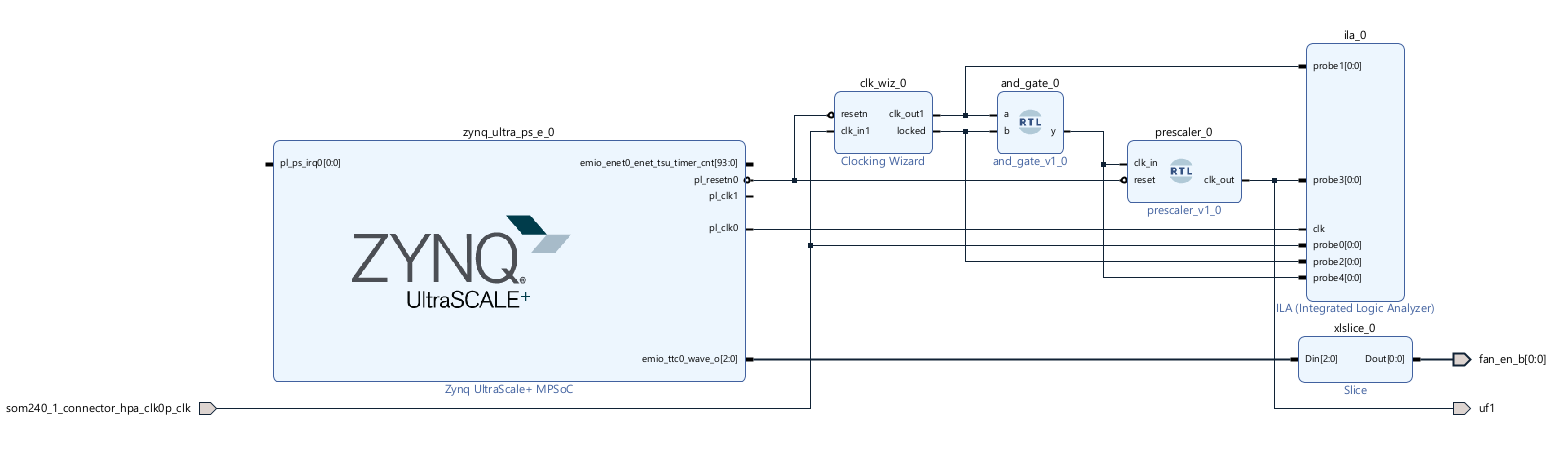
\includegraphics[width=1\textwidth]{images/prj3_1}
	\caption{Block scheme of the Vivado design.}
	\label{fig:prj3_1}
\end{figure}
Figure \ref{fig:prj3_1} presents a simple blinking LED design. In addition to the standard blocks imported from the example on which the design is based, the project includes several additional blocks required for proper functionality. Even though in the design is reported also the system processor block, the procedure will not deepen the Petalinux configuration, topic which will be touched in the next chapter.

\paragraph{Clocking Wizard} The Clocking Wizard is responsible for the generation of a 10 MHz clock source within the project. The IP is imported from the IP list of Vivado, thus no code is available for consultation. However, a block configuration procedure is needed to define the block behavior.

\paragraph{And Gate} The AND gate serves to create a stable clock source for the design by allowing the output only when the clocking wizard's output reaches a stable value. The VHDL implementation is given in the following code:
\vspace{0.1cm}
\begin{lstlisting}[language=VHDL]
library IEEE;
use IEEE.STD_LOGIC_1164.ALL;

entity and_gate is
	Port (a, b : in STD_LOGIC;
		    y : out STD_LOGIC);
end and_gate;

architecture Behavioral of and_gate is
begin
	y <= a and b;
end Behavioral;
\end{lstlisting}

\paragraph{Prescaler} The prescaler is used to further divide the clock frequency of the Clocking Wizard's output. Its output is directly connected to the LED, hence, to be visible, the frequency has to be smaller than few tens of Hz.
\vspace{0.1cm}
\begin{lstlisting}[language=VHDL]
-- Clock Divider
-- Every match, the output signal is toogled
-- The output frequency is given by: f_out = f_in / (2*max_val)

library IEEE;
use IEEE.STD_LOGIC_1164.ALL;
use IEEE.STD_LOGIC_ARITH.ALL;
use IEEE.STD_LOGIC_UNSIGNED.ALL;

entity prescaler is
	Port (clk_in, reset : in STD_LOGIC;
		    clk_out : out STD_LOGIC);
end prescaler;

architecture Behavioral of prescaler is
	constant max_val : integer := 500000;
	signal counter : integer range 0 to max_val-1 := 0;
	signal tmp : std_logic := '1';
begin
	process(clk_in, reset)
	begin
		if reset = '0'
		then
			tmp <= '0';
			counter <= 0;
		else
			if rising_edge(clk_in)
			then
				if counter = max_val-1 -- Counts from 0 to max_val-1
				then
					counter <= 0;
					tmp <= not tmp;
				else
					counter <= counter + 1;
				end if;
			end if;
		end if;
	end process;
clk_out <= tmp;
end Behavioral;
\end{lstlisting}

\paragraph{Integrated Logic Analyzer} This device acts like a digital oscilloscope and allows the displaying of the design internal signal that are connected to the blocks probes.




\subsection{Project creation}
The project was created, as aforementioned, starting from a design example. To create the project, open Vivado main page, click on \textbf{Open Example Project} → \textbf{Next} → \textbf{Kria Starter Kit Design Example} → select the KR260 board → rename the project → \textbf{Default Bitstream} → create the project. From the \textbf{Sources} windows delete the already existent wrapper, while keeping the design. To add the and gate and prescaler design blocks, move to \textbf{Sources} → \textbf{Design Sources} → right-click on this latter one → \textbf{Add Sources}.
\begin{figure}[h!t!]
	\centering
	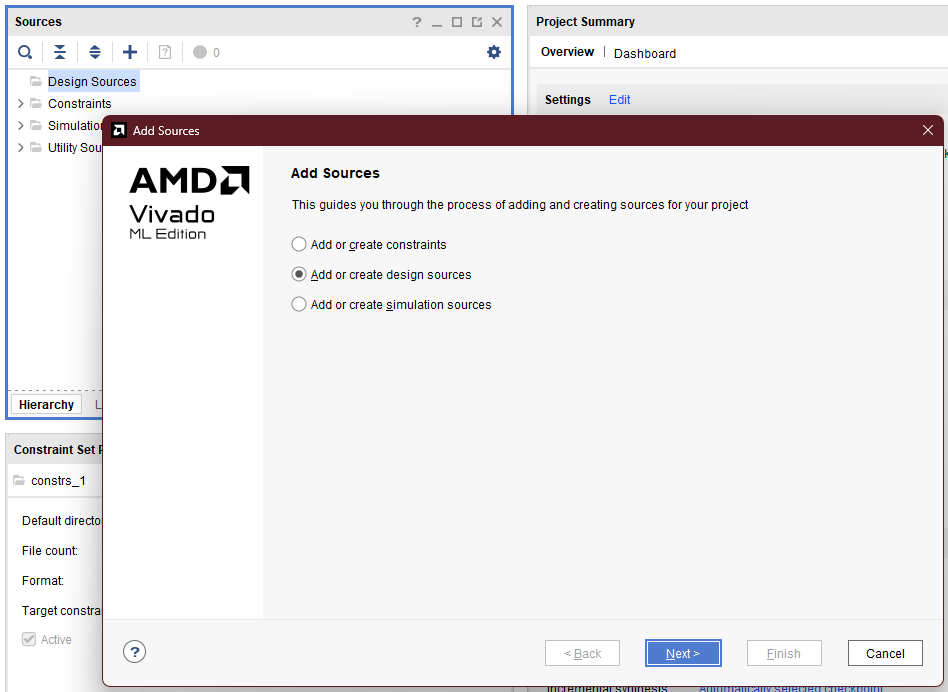
\includegraphics[width=0.8\textwidth]{images/vivado2}
	\caption{Block scheme of the Vivado design.}
	\label{fig:vivado2}
\end{figure}
Select \textbf{Add or create design sources} → \textbf{Next} → \textbf{Create file} → enter the file name → \textbf{Finish}. Once it
is done, a window to configure the inputs and the outputs of the gate should open. Such procedure can be skipped, providing that those information are defined in the description.

The Physical Constraint File (PCF) defines the mapping between the FPGA's internal logic and the physical pins of the development board. It specifies which FPGA pin is connected to which external component, such as LEDs, switches, or communication interfaces. This file is crucial for real-life applications, ensuring that the synthesized design correctly interfaces with the hardware. The process of defining physical constraints follows a procedure similar to the one used for behavioral descriptions (\textbf{Sources} → \textbf{Constraints} → right-click on this latter one → \textbf{Add Sources} → \textbf{Add or create constraints} → \textbf{Next} → \textbf{Create file} → enter the file name → \textbf{Finish}), but instead of describing logic functionality, it focuses on hardware connectivity and signal routing. Proper constraint definition prevents issues like incorrect signal assignment, which could lead to malfunctioning hardware or damage to the FPGA. The code to be written is:
\vspace{0.1cm}
\begin{lstlisting}[language=VHDL]
set_property BITSTREAM.GENERAL.COMPRESS TRUE [current_design]

#User defined pins
set_property PACKAGE_PIN F8 [get_ports {uf1}]
set_property IOSTANDARD LVCMOS18 [get_ports {uf1}]
\end{lstlisting}
\vspace{0.1cm}
A bit of explanation is needed to understand what these few lines of code do. The first line specifies that the bitstream generated for this project will be compressed, which helps reduce the file size, making it more efficient for storage and deployment. The subsequent lines define the physical connections between the FPGA and the hardware components (such as an LED) based on the datasheet of the development board. One line specifies that the LED is connected to a specific pin on the FPGA. This pin is defined as a standard I/O pin with a voltage logic of 1.8V (LVC-MOS18), which means that the pin uses Low Voltage CMOS (LVCMOS) logic at 1.8V to communicate with the LED. These settings ensure the correct functionality of the LED based on the voltage and current requirements of the board and peripheral components.


Under the section of \textbf{IP INTEGRATOR}, click on \textbf{Open Block Design}: a new window will open. Move back to \textbf{Design Sources} → right click on the description file(s) created earlier → \textbf{Add Module to Block Design}. To create a physical connection to the board pins, move the mouse tip on the block pins and type \textbf{Ctrl+T} to add a connection. By clicking on the created pins, a window named \textbf{External Port Properties} should appear. Rename those pins with the name defined in the constraints file. Click on the \textbf{+} sign on the top of the design window, search and add the clocking wizard IP block. Now the design should have the same blocks displayed in Figure \ref{fig:prj3_1}.

\subsection{Block configuration}
It should be now possible to run the automatic connection procedure (green tab on the top of the window). As previously explained, there is the necessity to configure the clocking wizard block (double click on the IP): set the reset to be active low, set the output clock to be the
value that you want (there is, however, a defined range of possible clock frequencies with specific values) and tick the section in which the input and output clock are in-phase. For this example the output frequency is set to be $f_{clk-wiz} = 10MHz$. With the prescaler VHDL code defined above, the clock frequency should be equal to
\begin{equation}
	f_{blink} = \frac{f_{clk-wiz}}{2ma_val} = 10Hz
\end{equation} 
Connect then the and gate, the prescaler and the ILA block as shown in Figure \ref{fig:prj3_1}.



\section{JTAG interface}
The Joint Test Action Group (JTAG) interface is primarily used for testing, debugging and programming FPGA devices during the development. It is a crucial tool in the development flow when working with Xilinx FPGAs, as it allows direct communication between a computer (running Vivado) and the FPGA. Its key features are a) FPGA programming, b)Debugging, c) Boundary-scan testing and d) Accessing internal signals (ILA core).

\subsection{JTAG programming}
To program the FPGA, a file similar to the .hex file used for programming uPs (e.g., ATmega, STM32) is required. However, for FPGA programming, this file is usually in the form of a bitstream file (commonly with extensions like .bit or .bin). The bitstream file contains the configuration data that programs the FPGA, mapping the logical design (created in VHDL, Verilog, or through a high-level tool like Vivado) onto the FPGA's hardware resources. Unlike microcontrollers, where code is executed sequentially, an FPGA is configured with a specific hardware design that defines the logic and behavior of the entire device. Move to the \textbf{PROGRAM AND DEBUG} section and click on \textbf{Generate Bitstream}. Follow the procedure and let the bitstream to be generated. The last step is to effectively program the device. Open the \textbf{Open Hardware Manager} and click on \textbf{Open Target} → \textbf{Auto Connect}, then click on \textbf{Program Device}.

\subsection{JTAG debugging}
After having programmed the FPGA, opene the \textbf{Hardware Manager} and connected the device, Vivado should automatically find the debug-probes file (if not, just re-program the FPGA). Between the various signals, chose one to be referred as trigger and define the trigger event (equal to a value, rising or falling edge...) and run the trigger event for the ILA core. A window similar to that of Figure \ref{fig:prj3_2} should appear.
\begin{figure}[h!t!]
	\centering
	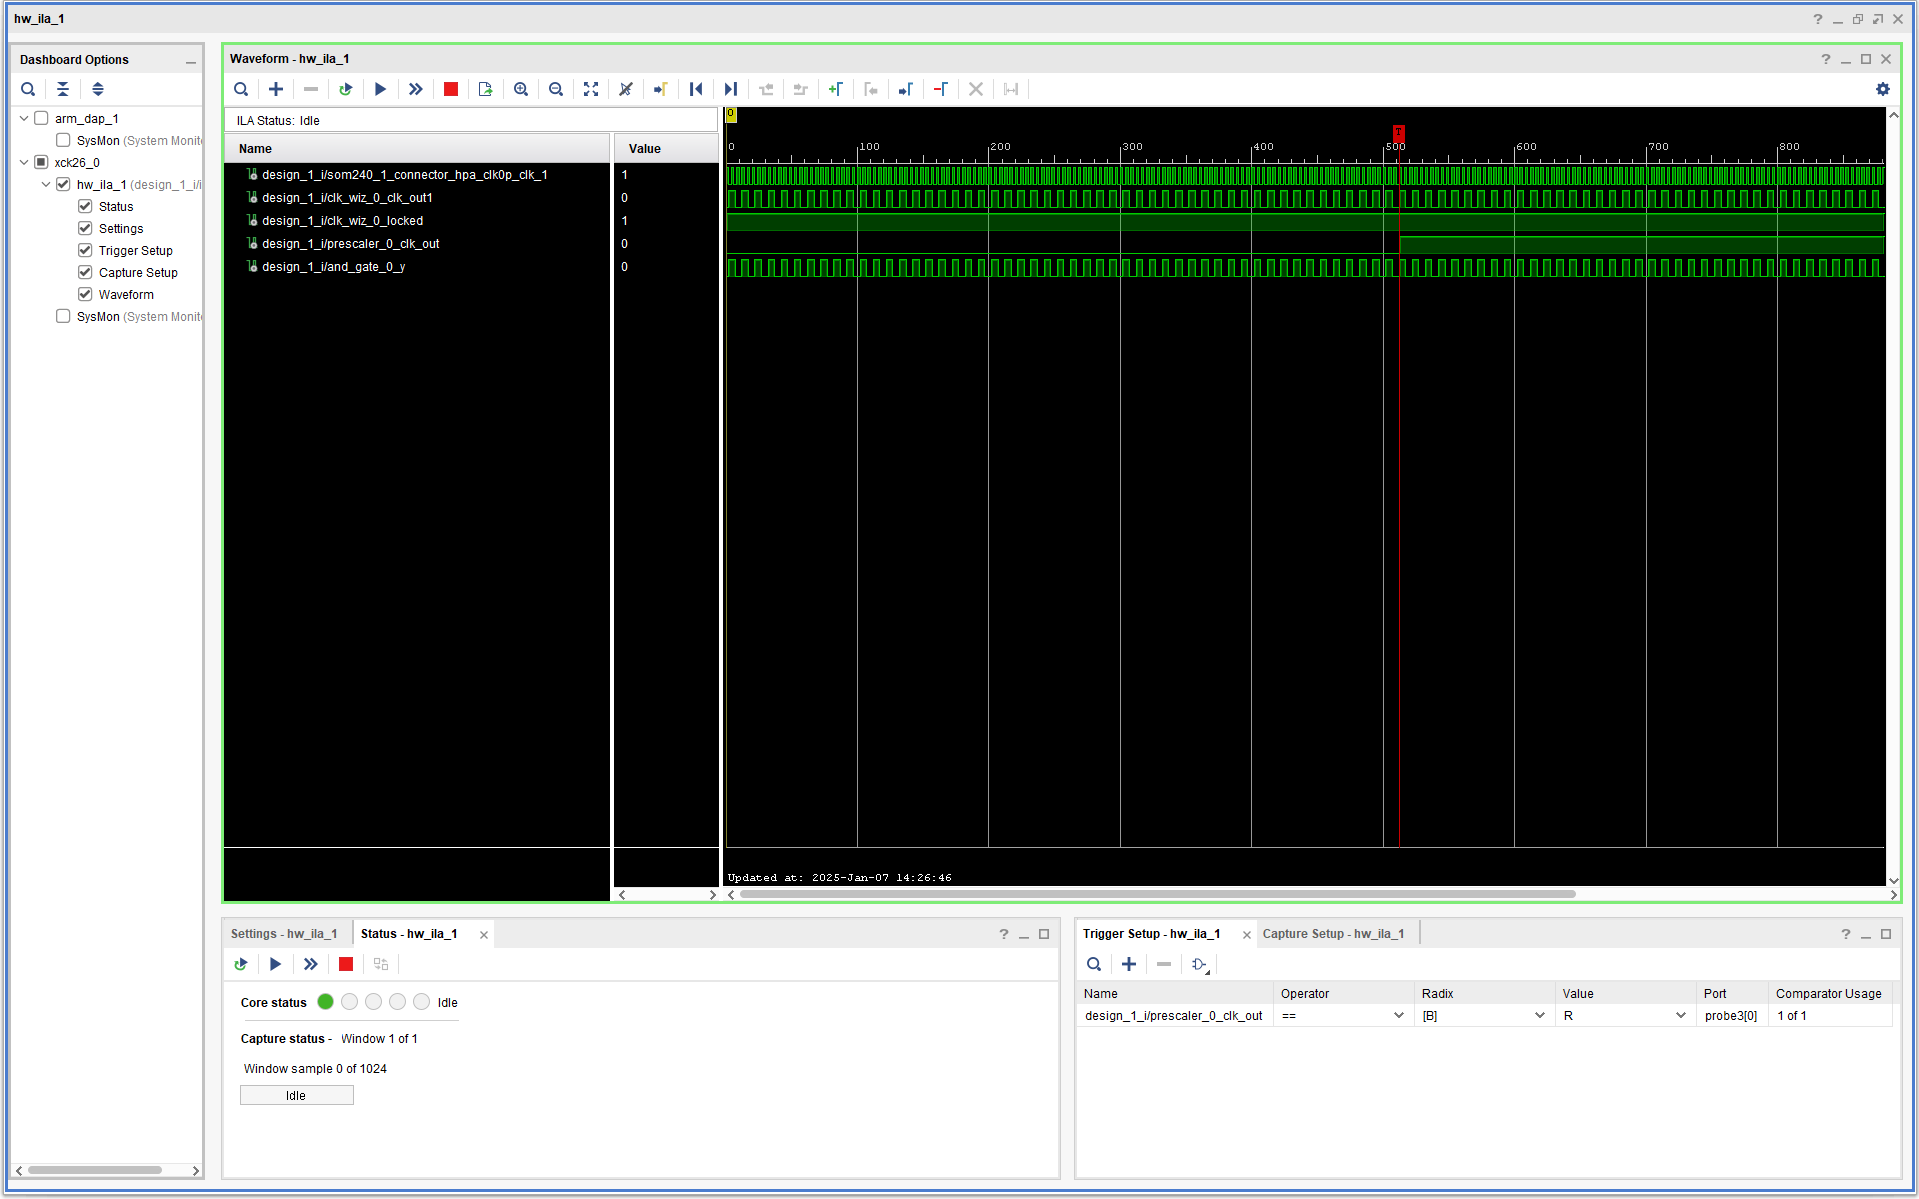
\includegraphics[width=0.8\textwidth]{images/prj3_2}
	\caption{J-tag debugging window.}
	\label{fig:prj3_2}
\end{figure}
	\chapter{Operative System Interface}
Once the fundamental process of programming the FPGA is understood, the next step is to explore how to fully exploit the capabilities of the SoM. This chapter provides a foundational overview, but it represents only a fraction of what can be achieved.

Within this chapter it is proposed the same blinking project, but the programming of the FPGA is performed directly by the uP. This latter steps need the configuration of a custom OS through Petalinux SDK. The system is said to be custom because at the end of the procedure, the OS will have enabled only the needed packages, thus it will results in a more lighter implementation with respect to an already available OS. To program the FPGA directly from the OS, a configuration file in a binary format is needed, thus the .bit file has to be converted. There are few ways to do so, but certainly the easiest is to add to the Vivado output the creation of the .bin file. From the previous project, go to \textbf{Settings} → \textbf{Bitstream} → \textbf{bin\_file} → \textbf{Apply} and regenerate the bistream. The .bin file should be saved in the same folder as the .bit file (\textit{project\_name/project\_name.runs/impl\_1}). In addition. also the hardware configuration file (.xsa) has to be generated (\textbf{File} → \textbf{Export} → \textbf{Export Hardware} → \textbf{Include Bitstream}). 

\section{Petalinux project}
From within the Petalinux installation folder type 
\vspace{0.1cm}
\begin{lstlisting}[language=bash]
	source ./settings.sh	
\end{lstlisting}
\vspace{0.1cm}
to initialize the environment. To create now the project related to the exported hardware file, type
\vspace{0.1cm}
\begin{lstlisting}[language=bash]
	petalinux-create --type project -s <path_to_bsp_file> --name <project_name>	
\end{lstlisting}
\vspace{0.1cm}
in which the .BSP file is saved in the same folder as the project and once it is done, move into the folder just created. The following two steps are quite important, so it is recommended to pay a bit more of attention.

\subsection{Hardware configuration}
The first configuration procedure aims to configure the core of the OS, i.e. to which architecture is addressed and which features are to be enabled. With the command
\vspace{0.1cm}
\begin{lstlisting}[language=bash]
	petalinux-config --get-hw-description <path_to_xsa_file>
\end{lstlisting}
\vspace{0.1cm}
a menu window will open (see Figure \ref{fig:prj2_2}), from which, moving into the various directories, the following packages must be enabled (or disabled):
\begin{itemize}
	\item \textbf{FPGA Manager $\rightarrow$ [*]FPGA Manager} (Enabled)
	\item \textbf{Image Packing Configuration $\rightarrow$ []Copy final images to tftpboot} (Disabled)
\end{itemize}
The FPGA manager will allow the FPGA to be programmed even during the operation of the board with few commands. However, during the creation of the image files, a warning message may appear stating that the .bit file wasn't loaded into the .wic image. To build the project type
\vspace{0.1cm}
\begin{lstlisting}[language=bash]
	petalinux-build	
\end{lstlisting}
\vspace{0.1cm}
\begin{figure}[h!t!]
	\centering
	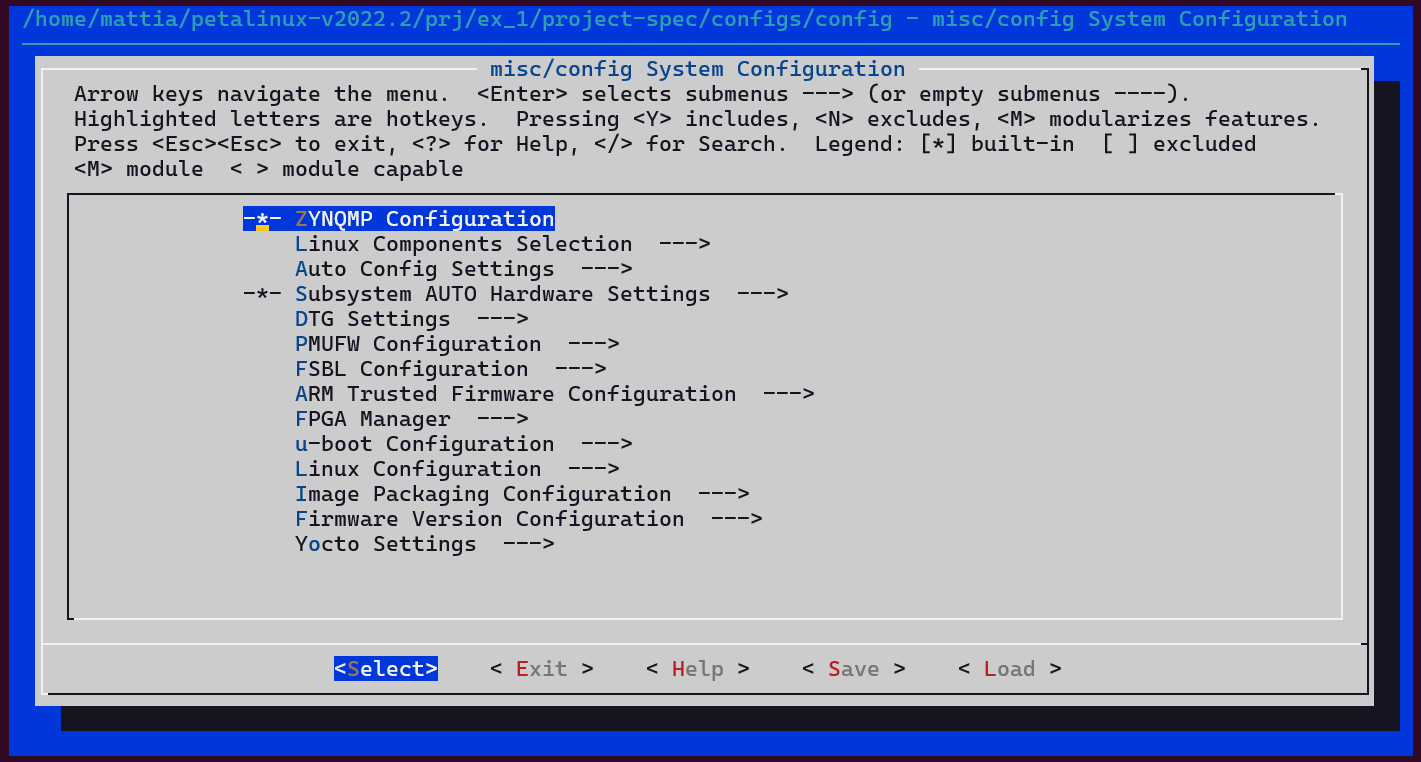
\includegraphics[width=0.8\textwidth]{images/prj2_2}
	\caption{Hardware configuration window.}
	\label{fig:prj2_2}
\end{figure}



\subsection{Packages configuration}
\label{subsec:rootfs-packages}
For the projects described in this guide, the root filesystem does not need the complete XRT/OpenCL acceleration stack. The target system must provide the basic Linux utilities, SSH access, native C/C++ compilation tools and the packages required to deploy custom FPGA applications based on FPGA Manager, device-tree overlays and kernel modules. Keeping the root filesystem minimal reduces both build time and image size.

The installation menu will open with the command
\vspace{0.1cm}
\begin{lstlisting}[language=bash]
	petalinux-config -c rootfs	
\end{lstlisting}
\vspace{0.1cm}
from which the following packages are recommended:
\begin{itemize}

	\item \textbf{Filesystem Packages} $\rightarrow$ \textbf{base} $\rightarrow$ \textbf{util-linux}
	
	\item \textbf{Filesystem Packages} $\rightarrow$ \textbf{console} $\rightarrow$ \textbf{utils} $\rightarrow$ \textbf{git} $\rightarrow$ \textbf{[*]git}
	
	\item \textbf{Filesystem Packages} $\rightarrow$ \textbf{console} $\rightarrow$ \textbf{utiles} $\rightarrow$ \textbf{strace}
	
	\item \textbf{Filesystem Packages} $\rightarrow$ \textbf{console} $\rightarrow$ \textbf{network} $\rightarrow$ \textbf{openssh} $\rightarrow$ \textbf{[*]openssh}, \textbf{[*]openssh-sshd}, \textbf{[*]openssh-sftp-server}
	
	\item \textbf{Filesystem Packages} $\rightarrow$ \textbf{misc} $\rightarrow$ \textbf{packagegroup-core-buildessential} $\rightarrow$ \textbf{[*]packagegroup-core-buildessential}
	
	\item \textbf{Filesystem Packages} $\rightarrow$ \textbf{misc} $\rightarrow$ \textbf{gcc-runtime} $\rightarrow$ \textbf{[*]libstdc++}
	
	\item \textbf{Filesystem Packages} $\rightarrow$ \textbf{misc} $\rightarrow$ \textbf{gdb} $\rightarrow$ \textbf{[*]gdb}
	
	\item \textbf{Filesystem Packages} $\rightarrow$ \textbf{misc} $\rightarrow$ \textbf{glibc} $\rightarrow$ \textbf{[*]glibc}, \textbf{[*]ldd}
	
	\item \textbf{PetaLinux Package Groups} $\rightarrow$ \textbf{packagegroup-petalinux} $\rightarrow$ \textbf{[*]packagegroup-petalinux}
\end{itemize}

This configuration provides the following features:
\begin{itemize}
	\item basic Linux command-line functionality;
	\item SSH remote access to the board;
	\item native C/C++ compilation directly on the KR260;
	\item basic debugging tools such as \texttt{gdb}, \texttt{dmesg} and \texttt{strace};
	\item FPGA Manager support for loading a \texttt{.bin} bitstream at run time;
	\item support for deploying device-tree overlays (\texttt{.dtbo});
	\item support for loading custom kernel modules (\texttt{.ko});
	\item support for the DMA-based user-space applications discussed in Chapter~\ref{ch:dma}.
\end{itemize}

The following packages are not required for the DMA implementation presented in this guide and can be disabled unless OpenCL/XRT acceleration, graphics or multimedia applications are explicitly needed:
\begin{itemize}
	\item \textbf{xrt}, \textbf{xrt-dev};
	\item \textbf{zocl};
	\item \textbf{opencl-headers};
	\item \textbf{opencl-clhpp}, \textbf{opencl-clhpp-dev};
	\item \textbf{libdrm}, \textbf{libdrm-tests}, \textbf{libdrm-kms};
	\item \textbf{bootgen}, \textbf{bootgen-dev};
	\item \textbf{dnf};
	\item \textbf{gcr}, \textbf{gcr-dev};
	\item \textbf{packagegroup-petalinux-gstreamer};
	\item \textbf{packagegroup-petalinux-opencv};
	\item \textbf{packagegroup-petalinux-v4lutils};
	\item \textbf{packagegroup-petalinux-x11}.
\end{itemize}

\begin{figure}[h!t!]
	\centering
	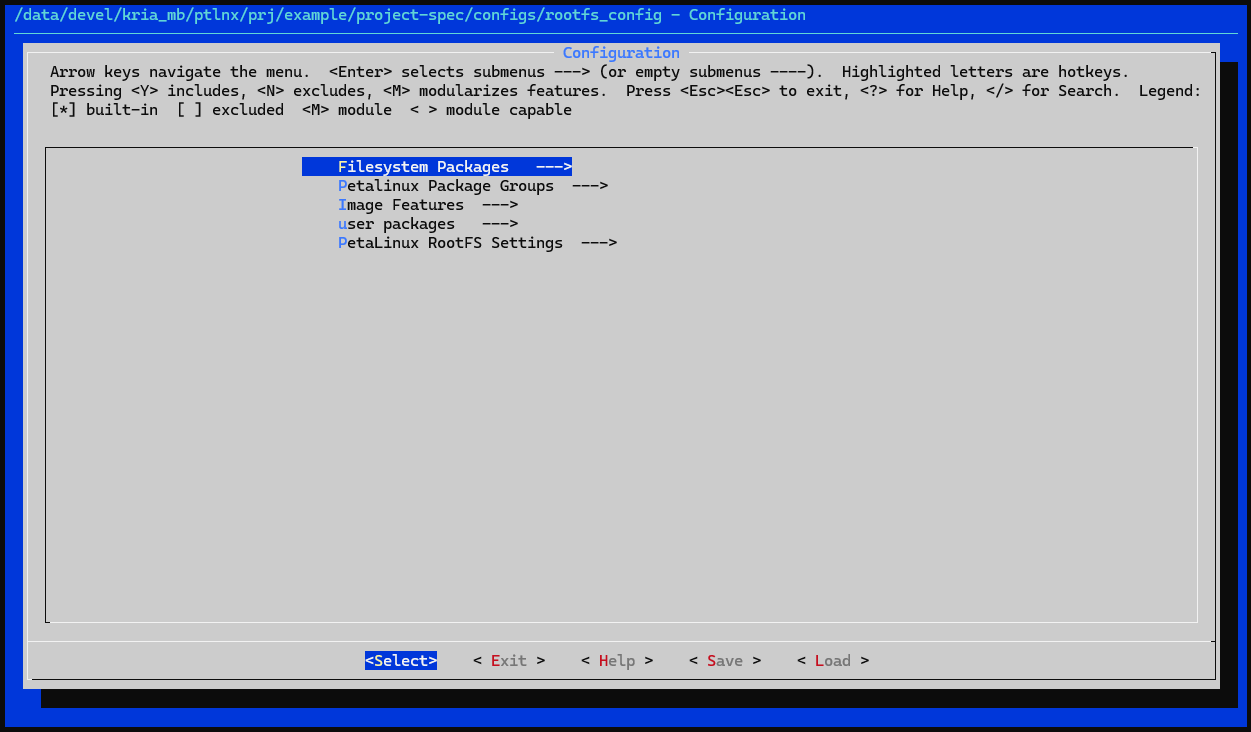
\includegraphics[width=0.8\textwidth]{images/prj2_3}
	\caption{rootfs configuration window.}
	\label{fig:prj2_3}
\end{figure}
After having installed all the needed packages, it is time to rebuild the project with the command
\vspace{0.1cm}
\begin{lstlisting}[language=bash]
	petalinux-build
\end{lstlisting}
\vspace{0.1cm}
In the case of building failure with error messages not related to the implementation, try to clear out the current files by typing
\vspace{0.1cm}
\begin{lstlisting}[language=bash]
	petalinux-config -x mrproper	
\end{lstlisting}
\vspace{0.1cm}
command which is used to deep cleaning the workspace, similar to how it's used in the Linux kernel build system.


\subsection{Board booting}
Since the board boots from a SD card, the system configuration just created has to be converted into a bootable image for the card itself. First step to carry out is the creation of the image files, which are then to be flashed into the SD card. To do so, after the project build, the command is (on the same line)
\vspace{0.1cm}
\begin{lstlisting}[language=bash]
	petalinux-package --boot --fsbl <zynqmp_fsbl.elf> --fpga <path_to_bitstream> --u-boot	
\end{lstlisting}
\vspace{0.1cm}
in which the .elf file is usually located under the path \textit{images/linux/}. The second step is to create a .wic image for the SD card to be flashed in. The command to do that is (on the same line)
\vspace{0.1cm}
\begin{lstlisting}[language=bash]
	petalinux-package --wic --images-dir images/linux/ --bootfiles "ramdisk.cpio.gz.u-boot,boot.scr,Image,system.dtb,system-zynqmp-sck-kr-g-revB.dtb" --disk-name "sda"	
\end{lstlisting}
\vspace{0.1cm}
from which the .wic image will be generated and found in the same folder as the .elf file. To flash the SD card make use of a third-part software, such as balenaEtcher or something similar. Once the flash is done, insert the SD in the board and power it up. With a third part software, such as PuTTY, connect to the serial port (Baud Rate 115200). The system will require to inset some credential. 


\subsection{SSH connection}
Once the board is connected through a serial terminal and the Ethernet cable is plugged in, it is possible to find out the IP address associated to the device by typing
\vspace{0.1cm}
\begin{lstlisting}[language=bash]
	ip a
\end{lstlisting}
\vspace{0.1cm}
Once the IP is known, it is possible to connect to the board via SSH protocol:
\vspace{0.1cm}
\begin{lstlisting}[language=bash]
	ssh board_name@ip_address
\end{lstlisting}
\vspace{0.1cm}


\section{FPGA programming}
So far, the FPGA is not yet programmed. Besides the JTAG procedure, also the On-Run programming is of use: it allows for more flexibility and has the advantage to let the FPGA to be programmed even when the system is running, without the need to repeat all the steps previously explained. To actually program the FPGA after the system is booted, there is the need to the .bin file needs to be "manually" loaded into the FPGA through the FPGA manager. Through SSH copy the .bin file in the /lib/firmware path and to program the FPGA type 
\begin{lstlisting}[language=bash]
	sudo sh -c 'echo "bin_file" > /sys/class/fpga_manager/fpga0/firmware'	\end{lstlisting}
The .bin file can be automatically generated by Vivado when writing the bitstream file. Go to \textbf{Settings}, then \textbf{Bitstream} and check the .bin box.
	%\chapter{Memory operations}



\section{Vivado project}
The Vivado block scheme of the project is shown in Figure \ref{fig:fifo}. 
\begin{figure}[h!t!]
	\centering
	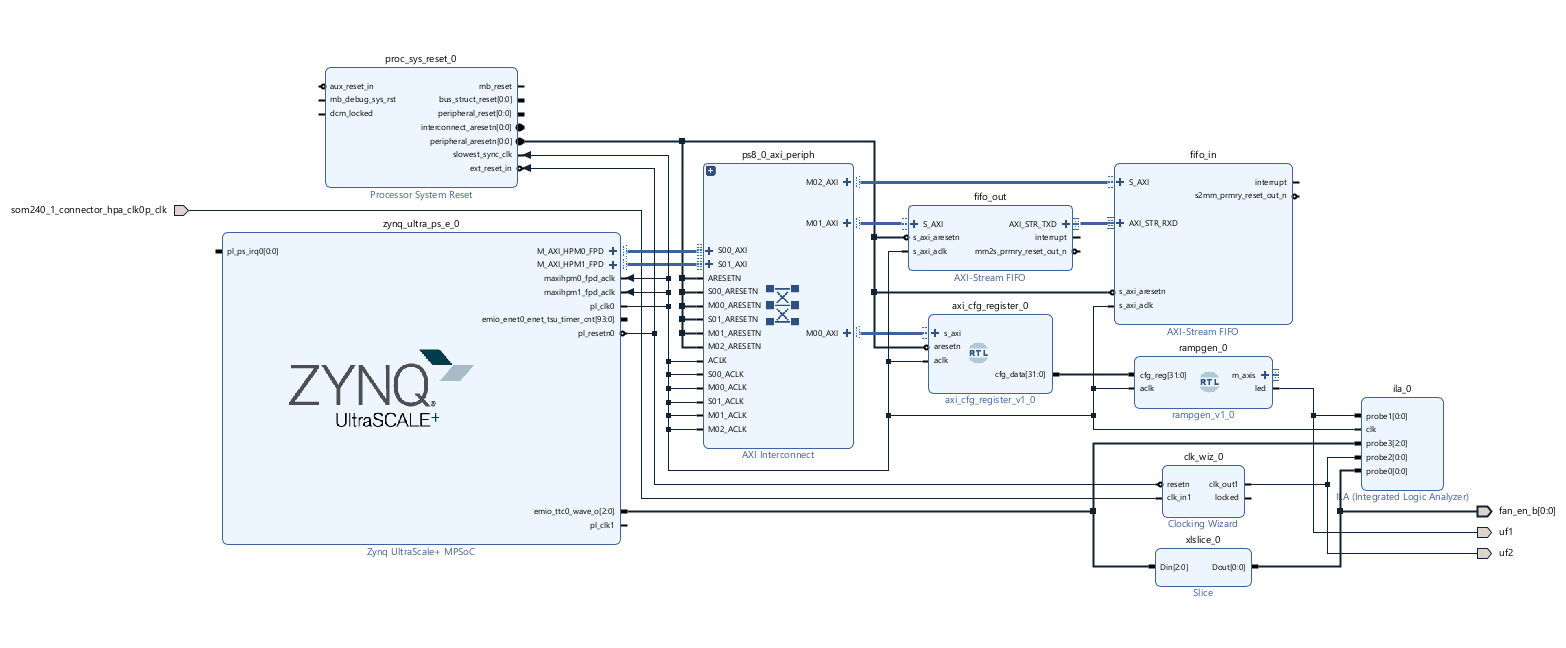
\includegraphics[width=1\textwidth]{images/fifo}
	\caption{Block scheme of the memory operation design project.}
	\label{fig:fifo}
\end{figure}
It is easy to notice that this implementation is more complex than the previous one. In addition to the previously used IP blocks, a few more have been added to enhance functionality. These additional components play a crucial role in enabling efficient data exchange and communication between the Processing System (PS) and Programmable Logic (PL), making the design more sophisticated and capable.

\subsection{Block description}
\paragraph{AXI Interconnect \& Processor System Reset}
These two blocks are automatically imported when the automatic interconnection process is initiated. As a result, there is no need to manually define any code for their integration, as they are handled by the system's design automation tools. The former block facilitates communication between the PS and PL by managing data transfers over the Advanced eXtensible Interface (AXI) protocol. It connects multiple AXI peripherals and ensures efficient data routing. The second block handles the reset signals for the entire system, ensuring that the processor and connected peripherals start in a known, stable state during initialization or after a reset event.

\paragraph{rampgen\_v1.0}
This building block serve to generate the test signal to be written/read by/in the FIFO memories. However, in the current implementation, such block is not used and the data generation is handled directly via software. However, its code is shown below.
\vspace{0.1cm}
\begin{lstlisting}[language=VHDL]
library IEEE;
use ieee.std_logic_1164.all;
use ieee.numeric_std.all;
use ieee.std_logic_misc.all;

entity rampgen is
	Port ( 
	aclk : in STD_LOGIC;
	cfg_reg : in STD_LOGIC_VECTOR (31 downto 0);
	m_axis_tdata        : out std_logic_vector(31 downto 0);
	m_axis_tvalid       : out std_logic;
	m_axis_tready       : in  std_logic;
	m_axis_tlast        : out std_logic;
	led : out STD_LOGIC);
end rampgen;

architecture implementation of rampgen is
	signal prev_reg: STD_LOGIC_VECTOR (31 downto 0);
	signal led_out: STD_LOGIC := '0';
begin
	led <= led_out;
	handle_ramp: process(aclk)
		variable out_count : integer;
	begin
		if rising_edge(aclk)  
		then
			if (prev_reg = "00000000000000000000000000000000" and not (cfg_reg =  "00000000000000000000000000000000")) 
			then 
				out_count := to_integer(signed(cfg_reg(31 downto 0)));
				led_out <= '1';
			end if;
			if out_count > 0 and m_axis_tready = '1' 
			then
				out_count := out_count - 1;
				m_axis_tdata <= std_logic_vector(to_unsigned(out_count, 32));
				m_axis_tvalid <= '1';
				m_axis_tlast <= '1';
			else
				m_axis_tvalid <= '0';
				m_axis_tlast <= '0';
			end if;
			prev_reg <= cfg_reg;
		end if;
	end process; 
end implementation;
\end{lstlisting}

\paragraph{axi\_cfg\_register}
This register facilitates communication between the user and the device. Although it is not utilized in the current implementation, it was previously used to set the initial value for the ramp generator. Its code is reported below.
\vspace{0.1cm}
\begin{lstlisting}[language=Verilog]
`timescale 1 ns / 1 ps

module axi_cfg_register #
(
	parameter integer CFG_DATA_WIDTH = 1024,
	parameter integer AXI_DATA_WIDTH = 32,
	parameter integer AXI_ADDR_WIDTH = 32
)
(
	// System signals
	input  wire                        aclk,
	input  wire                        aresetn,
	
	// Configuration bits
	output wire [CFG_DATA_WIDTH-1:0]   cfg_data,
	
	// Slave side
	input  wire [AXI_ADDR_WIDTH-1:0]   s_axi_awaddr,  // AXI4-Lite slave: Write address
	input  wire                        s_axi_awvalid, // AXI4-Lite slave: Write address valid
	output wire                        s_axi_awready, // AXI4-Lite slave: Write address ready
	input  wire [AXI_DATA_WIDTH-1:0]   s_axi_wdata,   // AXI4-Lite slave: Write data
	input  wire [AXI_DATA_WIDTH/8-1:0] s_axi_wstrb,   // AXI4-Lite slave: Write strobe
	input  wire                        s_axi_wvalid,  // AXI4-Lite slave: Write data valid
	output wire                        s_axi_wready,  // AXI4-Lite slave: Write data ready
	output wire [1:0]                  s_axi_bresp,   // AXI4-Lite slave: Write response
	output wire                        s_axi_bvalid,  // AXI4-Lite slave: Write response valid
	input  wire                        s_axi_bready,  // AXI4-Lite slave: Write response ready
	input  wire [AXI_ADDR_WIDTH-1:0]   s_axi_araddr,  // AXI4-Lite slave: Read address
	input  wire                        s_axi_arvalid, // AXI4-Lite slave: Read address valid
	output wire                        s_axi_arready, // AXI4-Lite slave: Read address ready
	output wire [AXI_DATA_WIDTH-1:0]   s_axi_rdata,   // AXI4-Lite slave: Read data
	output wire [1:0]                  s_axi_rresp,   // AXI4-Lite slave: Read data response
	output wire                        s_axi_rvalid,  // AXI4-Lite slave: Read data valid
	input  wire                        s_axi_rready   // AXI4-Lite slave: Read data ready
);

function integer clogb2 (input integer value);
	for(clogb2 = 0; value > 0; clogb2 = clogb2 + 1) value = value >> 1;
endfunction

localparam integer ADDR_LSB = clogb2(AXI_DATA_WIDTH/8 - 1);
localparam integer CFG_SIZE = CFG_DATA_WIDTH/AXI_DATA_WIDTH;
localparam integer CFG_WIDTH = CFG_SIZE > 1 ? clogb2(CFG_SIZE-1) : 1;

reg int_bvalid_reg, int_bvalid_next;

reg int_rvalid_reg, int_rvalid_next;
reg [AXI_DATA_WIDTH-1:0] int_rdata_reg, int_rdata_next;

wire [AXI_DATA_WIDTH-1:0] int_data_mux [CFG_SIZE-1:0];
wire [CFG_DATA_WIDTH-1:0] int_data_wire;
wire [CFG_SIZE-1:0] int_ce_wire;
wire int_wvalid_wire;

genvar j, k;

assign int_wvalid_wire = s_axi_awvalid & s_axi_wvalid;

generate
	for(j = 0; j < CFG_SIZE; j = j + 1)
	begin : WORDS
		assign int_data_mux[j] = int_data_wire[j*AXI_DATA_WIDTH+AXI_DATA_WIDTH-1:j*AXI_DATA_WIDTH];
		assign int_ce_wire[j] = int_wvalid_wire & (s_axi_awaddr[ADDR_LSB+CFG_WIDTH-1:ADDR_LSB] == j);
		for(k = 0; k < AXI_DATA_WIDTH; k = k + 1)
			begin : BITS
			FDRE #(
			.INIT(1'b0)
			) FDRE_inst (
			.CE(int_ce_wire[j] & s_axi_wstrb[k/8]),
			.C(aclk),
			.R(~aresetn),
			.D(s_axi_wdata[k]),
			.Q(int_data_wire[j*AXI_DATA_WIDTH + k])
			);
		end
	end
endgenerate

always @(posedge aclk)
begin
	if(~aresetn)
		begin
			int_bvalid_reg <= 1'b0;
			int_rvalid_reg <= 1'b0;
			int_rdata_reg <= {(AXI_DATA_WIDTH){1'b0}};
		end
		else
		begin
			int_bvalid_reg <= int_bvalid_next;
			int_rvalid_reg <= int_rvalid_next;
			int_rdata_reg <= int_rdata_next;
	end
end

always @*
begin
	int_bvalid_next = int_bvalid_reg;
	
	if(int_wvalid_wire)
	begin
		int_bvalid_next = 1'b1;
	end
	
	if(s_axi_bready & int_bvalid_reg)
	begin
		int_bvalid_next = 1'b0;
	end
end

always @*
begin
	int_rvalid_next = int_rvalid_reg;
	int_rdata_next = int_rdata_reg;
	
	if(s_axi_arvalid)
	begin
		int_rvalid_next = 1'b1;
		int_rdata_next = int_data_mux[s_axi_araddr[ADDR_LSB+CFG_WIDTH-1:ADDR_LSB]];
	end
	
	if(s_axi_rready & int_rvalid_reg)
	begin
		int_rvalid_next = 1'b0;
	end
end

assign cfg_data = int_data_wire;

assign s_axi_bresp = 2'd0;
assign s_axi_rresp = 2'd0;

assign s_axi_awready = int_wvalid_wire;
assign s_axi_wready = int_wvalid_wire;
assign s_axi_bvalid = int_bvalid_reg;
assign s_axi_arready = 1'b1;
assign s_axi_rdata = int_rdata_reg;
assign s_axi_rvalid = int_rvalid_reg;

endmodule
\end{lstlisting}


\paragraph{FIFO IN \& FIFO OUT}
The two First-In, First-Out (FIFO) memory blocks are configured separately—one for input and one for output. These blocks are selected from the IP block catalog in Vivado and integrated into the design. The FIFO OUT memory is responsible for writing data into the FIFO IN memory. Then, the written data is read via software and simply printed in the terminal window, demonstrating the (hopefully) successful communication between the FPGA and the processing system.


\subsection{Block configuration}
The project described in this chapter demonstrates the ability to read and write data within memory blocks defined in the FPGA through an interface between PL and PS. The register and FIFO memories allocate a specific amount of memory to store the data. The address is automatically assigned in the Vivado \textbf{ADDRESS EDITOR}, as shown in Figure \ref{fig:addresses}, though manual adjustments may be necessary.
\begin{figure}[h!t!]
	\centering
	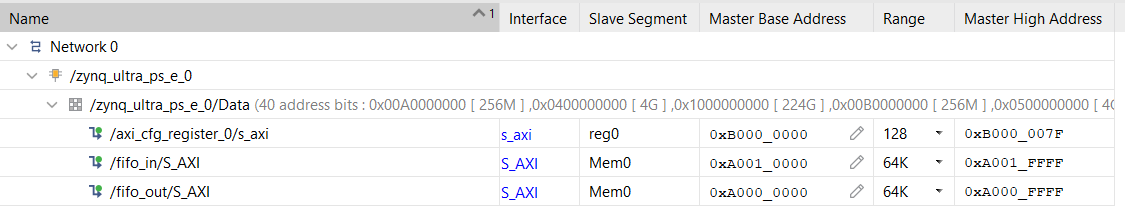
\includegraphics[width=1\textwidth]{images/addresses}
	\caption{Addresses definition.}
	\label{fig:addresses}
\end{figure}
The receive/transmit FIFO depth was set to 2048 byte. Regarding the other blocks, their configuration does not require any additional steps beyond what was covered in the previous chapters. Similarly, the generation of the bitstream and the .bin file follows the same process and does not require further explanation.



\section{Petalinux project}
The configuration of the PetaLinux project remains the same as explained in the previous chapter up to the rootfs configuration. However, when creating the driver, certain files need to be modified, requiring an update of the project. These modifications ensure the proper integration of the new software components.



\section{Driver implementation}
After successfully building the project, performing read/write operations on the memories and registers requires the definition of two additional components: a) the Driver, responsible for managing communication between the PS and the PL and b) the user program, which executes the operations using the driver to interact with the hardware. The driver must then be compiled into a .ko (Kernel Object) file, which can be loaded and executed on the KRIA board. The procedure to achieve this is quite complex, and even small mistakes can lead to errors. Therefore, careful attention is required at each step to ensure successful implementation.



The first step is to locate two files:
\begin{itemize}
	\item \textbf{system-user.dtsi} (found in \textit{project-spe/meta-user/recipes-bps/device-tree/files})
	
	\item \textbf{pl.dtsi} )
\end{itemize}
and open them with an editor. Down below is reported the code of pl.dtsi.
\vspace{0.1cm}
\begin{lstlisting}[language=C]
/dts-v1/;
/plugin/;
/ {
	fragment@0 {
		target = <&fpga_full>;
		overlay0: __overlay__ {
			#address-cells = <2>;
			#size-cells = <2>;
			firmware-name = "design_1_wrapper.bit.bin";
			resets = <&zynqmp_reset 116>;
		};
	};
	fragment@1 {
		target = <&amba>;
		overlay1: __overlay__ {
			afi0: afi0 {
				compatible = "xlnx,afi-fpga";
				config-afi = < 0 0>, <1 0>, <2 0>, <3 0>, <4 0>, <5 0>, <6 0>, <7 0>, <8 0>, <9 0>, <10 0>, <11 0>, <12 0>, <13 0>, <14 0xa00>, <15 0x000>;
			};
			clocking0: clocking0 {
				#clock-cells = <0>;
				assigned-clock-rates = <99999001>;
				assigned-clocks = <&zynqmp_clk 71>;
				clock-output-names = "fabric_clk";
				clocks = <&zynqmp_clk 71>;
				compatible = "xlnx,fclk";
			};
			clocking1: clocking1 {
				#clock-cells = <0>;
				assigned-clock-rates = <99999001>;
				assigned-clocks = <&zynqmp_clk 72>;
				clock-output-names = "fabric_clk";
				clocks = <&zynqmp_clk 72>;
				compatible = "xlnx,fclk";
			};
		};
	};
	fragment@2 {
		target = <&amba>;
		overlay2: __overlay__ {
			#address-cells = <2>;
			#size-cells = <2>;
			axi_cfg_register_0: axi_cfg_register@b0000000 {
				clock-names = "aclk";
				clocks = <&zynqmp_clk 71>;
				compatible = "xlnx,axi-cfg-register-1.0";
				reg = <0x0 0xb0000000 0x0 0x80>;
			};
			fifo_in: axi_fifo_mm_s@a0010000 {
				clock-names = "s_axi_aclk";
				clocks = <&zynqmp_clk 71>;
				compatible = "xlnx,axi-fifo-mm-s-4.3";
				reg = <0x0 0xa0010000 0x0 0x10000>;
				xlnx,axi-str-rxd-protocol = "XIL_AXI_STREAM_ETH_DATA";
				xlnx,axi-str-rxd-tdata-width = <0x20>;
				xlnx,axi-str-txc-protocol = "XIL_AXI_STREAM_ETH_CTRL";
				xlnx,axi-str-txc-tdata-width = <0x20>;
				xlnx,axi-str-txd-protocol = "XIL_AXI_STREAM_ETH_DATA";
				xlnx,axi-str-txd-tdata-width = <0x20>;
				xlnx,axis-tdest-width = <0x4>;
				xlnx,axis-tid-width = <0x4>;
				xlnx,axis-tuser-width = <0x4>;
				xlnx,data-interface-type = <0x0>;
				xlnx,has-axis-tdest = <0x0>;
				xlnx,has-axis-tid = <0x0>;
				xlnx,has-axis-tkeep = <0x0>;
				xlnx,has-axis-tstrb = <0x0>;
				xlnx,has-axis-tuser = <0x0>;
				xlnx,rx-cascade-height = <0x0>;
				xlnx,rx-enable-ecc = <0x0>;
				xlnx,rx-fifo-depth = <0x800>;
				xlnx,rx-fifo-pe-threshold = <0x5>;
				xlnx,rx-fifo-pf-threshold = <0x1fb>;
				xlnx,rx-has-ecc-err-inject = <0x0>;
				xlnx,s-axi-id-width = <0x4>;
				xlnx,s-axi4-data-width = <0x20>;
				xlnx,select-xpm = <0x0>;
				xlnx,tx-cascade-height = <0x0>;
				xlnx,tx-enable-ecc = <0x0>;
				xlnx,tx-fifo-depth = <0x200>;
				xlnx,tx-fifo-pe-threshold = <0x5>;
				xlnx,tx-fifo-pf-threshold = <0x1fb>;
				xlnx,tx-has-ecc-err-inject = <0x0>;
				xlnx,use-rx-cut-through = <0x0>;
				xlnx,use-rx-data = <0x1>;
				xlnx,use-tx-ctrl = <0x0>;
				xlnx,use-tx-cut-through = <0x0>;
				xlnx,use-tx-data = <0x0>;
			};
			fifo_out: axi_fifo_mm_s@a0000000 {
				clock-names = "s_axi_aclk";
				clocks = <&zynqmp_clk 71>;
				compatible = "xlnx,axi-fifo-mm-s-4.3";
				reg = <0x0 0xa0000000 0x0 0x10000>;
				xlnx,axi-str-rxd-protocol = "XIL_AXI_STREAM_ETH_DATA";
				xlnx,axi-str-rxd-tdata-width = <0x20>;
				xlnx,axi-str-txc-protocol = "XIL_AXI_STREAM_ETH_CTRL";
				xlnx,axi-str-txc-tdata-width = <0x20>;
				xlnx,axi-str-txd-protocol = "XIL_AXI_STREAM_ETH_DATA";
				xlnx,axi-str-txd-tdata-width = <0x20>;
				xlnx,axis-tdest-width = <0x4>;
				xlnx,axis-tid-width = <0x4>;
				xlnx,axis-tuser-width = <0x4>;
				xlnx,data-interface-type = <0x0>;
				xlnx,has-axis-tdest = <0x0>;
				xlnx,has-axis-tid = <0x0>;
				xlnx,has-axis-tkeep = <0x0>;
				xlnx,has-axis-tstrb = <0x0>;
				xlnx,has-axis-tuser = <0x0>;
				xlnx,rx-cascade-height = <0x0>;
				xlnx,rx-enable-ecc = <0x0>;
				xlnx,rx-fifo-depth = <0x200>;
				xlnx,rx-fifo-pe-threshold = <0x5>;
				xlnx,rx-fifo-pf-threshold = <0x1fb>;
				xlnx,rx-has-ecc-err-inject = <0x0>;
				xlnx,s-axi-id-width = <0x4>;
				xlnx,s-axi4-data-width = <0x20>;
				xlnx,select-xpm = <0x0>;
				xlnx,tx-cascade-height = <0x0>;
				xlnx,tx-enable-ecc = <0x0>;
				xlnx,tx-fifo-depth = <0x800>;
				xlnx,tx-fifo-pe-threshold = <0x5>;
				xlnx,tx-fifo-pf-threshold = <0x1fb>;
				xlnx,tx-has-ecc-err-inject = <0x0>;
				xlnx,use-rx-cut-through = <0x0>;
				xlnx,use-rx-data = <0x0>;
				xlnx,use-tx-ctrl = <0x1>;
				xlnx,use-tx-cut-through = <0x0>;
				xlnx,use-tx-data = <0x1>;
			};
		};
	};
};
\end{lstlisting}
\vspace{0.1cm}
Edit the system-user.dtsi file, which is initially empty, by creating the \textbf{amba\_pl} device tree node. Within this node: a) copy the afi node, b) include all components related to the memories instantiated in the Vivado design and c) copy the \textbf{clocking0} and \textbf{clocking1} components. The final system-user.dtsi file for this application is shown below.
\vspace{0.1cm}
\begin{lstlisting}[language=C]
/include/ "system-conf.dtsi"
/ {
	amba_pl: amba_pl {
		compatible = "simple-bus";
		ranges ;
		axi_cfg_register_0: axi_cfg_register@b0000000 {
			clock-names = "aclk";
			clocks = <&zynqmp_clk 71>;
			compatible = "xlnx,axi-cfg-register-1.0";
			reg = <0x0 0xb0000000 0x0 0x80>;
		};
		afi0: afi0 {
			compatible = "xlnx,afi-fpga";
			config-afi = < 0 0>, <1 0>, <2 0>, <3 0>, <4 0>, <5 0>, <6 0>, <7 0>, <8 0>, <9 0>, <10 0>, <11 0>, <12 0>, <13 0>, <14 0xa00>, <15 0x000>;
		};
		clocking0: clocking0 {
			#clock-cells = <0>;
			assigned-clock-rates = <99999001>;
			assigned-clocks = <&zynqmp_clk 71>;
			clock-output-names = "fabric_clk";
			clocks = <&zynqmp_clk 71>;
			compatible = "xlnx,fclk";
		};
		clocking1: clocking1 {
			#clock-cells = <0>;
			assigned-clock-rates = <99999001>;
			assigned-clocks = <&zynqmp_clk 72>;
			clock-output-names = "fabric_clk";
			clocks = <&zynqmp_clk 72>;
			compatible = "xlnx,fclk";
		};
		fifo_in: axi_fifo_mm_s@a0010000 {
			clock-names = "s_axi_aclk";
			clocks = <&zynqmp_clk 71>;
			compatible = "xlnx,axi-fifo-mm-s-4.3";
			reg = <0x0 0xa0010000 0x0 0x10000>;
			xlnx,axi-str-rxd-protocol = "XIL_AXI_STREAM_ETH_DATA";
			xlnx,axi-str-rxd-tdata-width = <0x20>;
			xlnx,axi-str-txc-protocol = "XIL_AXI_STREAM_ETH_CTRL";
			xlnx,axi-str-txc-tdata-width = <0x20>;
			xlnx,axi-str-txd-protocol = "XIL_AXI_STREAM_ETH_DATA";
			xlnx,axi-str-txd-tdata-width = <0x20>;
			xlnx,axis-tdest-width = <0x4>;
			xlnx,axis-tid-width = <0x4>;
			xlnx,axis-tuser-width = <0x4>;
			xlnx,data-interface-type = <0x0>;
			xlnx,has-axis-tdest = <0x0>;
			xlnx,has-axis-tid = <0x0>;
			xlnx,has-axis-tkeep = <0x0>;
			xlnx,has-axis-tstrb = <0x0>;
			xlnx,has-axis-tuser = <0x0>;
			xlnx,rx-cascade-height = <0x0>;
			xlnx,rx-enable-ecc = <0x0>;
			xlnx,rx-fifo-depth = <0x800>;
			xlnx,rx-fifo-pe-threshold = <0x5>;
			xlnx,rx-fifo-pf-threshold = <0x1fb>;
			xlnx,rx-has-ecc-err-inject = <0x0>;
			xlnx,s-axi-id-width = <0x4>;
			xlnx,s-axi4-data-width = <0x20>;
			xlnx,select-xpm = <0x0>;
			xlnx,tx-cascade-height = <0x0>;
			xlnx,tx-enable-ecc = <0x0>;
			xlnx,tx-fifo-depth = <0x200>;
			xlnx,tx-fifo-pe-threshold = <0x5>;
			xlnx,tx-fifo-pf-threshold = <0x1fb>;
			xlnx,tx-has-ecc-err-inject = <0x0>;
			xlnx,use-rx-cut-through = <0x0>;
			xlnx,use-rx-data = <0x1>;
			xlnx,use-tx-ctrl = <0x0>;
			xlnx,use-tx-cut-through = <0x0>;
			xlnx,use-tx-data = <0x0>;
		};
		fifo_out: axi_fifo_mm_s@a0000000 {
			clock-names = "s_axi_aclk";
			clocks = <&zynqmp_clk 71>;
			compatible = "xlnx,axi-fifo-mm-s-4.3";
			reg = <0x0 0xa0000000 0x0 0x10000>;
			xlnx,axi-str-rxd-protocol = "XIL_AXI_STREAM_ETH_DATA";
			xlnx,axi-str-rxd-tdata-width = <0x20>;
			xlnx,axi-str-txc-protocol = "XIL_AXI_STREAM_ETH_CTRL";
			xlnx,axi-str-txc-tdata-width = <0x20>;
			xlnx,axi-str-txd-protocol = "XIL_AXI_STREAM_ETH_DATA";
			xlnx,axi-str-txd-tdata-width = <0x20>;
			xlnx,axis-tdest-width = <0x4>;
			xlnx,axis-tid-width = <0x4>;
			xlnx,axis-tuser-width = <0x4>;
			xlnx,data-interface-type = <0x0>;
			xlnx,has-axis-tdest = <0x0>;
			xlnx,has-axis-tid = <0x0>;
			xlnx,has-axis-tkeep = <0x0>;
			xlnx,has-axis-tstrb = <0x0>;
			xlnx,has-axis-tuser = <0x0>;
			xlnx,rx-cascade-height = <0x0>;
			xlnx,rx-enable-ecc = <0x0>;
			xlnx,rx-fifo-depth = <0x200>;
			xlnx,rx-fifo-pe-threshold = <0x5>;
			xlnx,rx-fifo-pf-threshold = <0x1fb>;
			xlnx,rx-has-ecc-err-inject = <0x0>;
			xlnx,s-axi-id-width = <0x4>;
			xlnx,s-axi4-data-width = <0x20>;
			xlnx,select-xpm = <0x0>;
			xlnx,tx-cascade-height = <0x0>;
			xlnx,tx-enable-ecc = <0x0>;
			xlnx,tx-fifo-depth = <0x800>;
			xlnx,tx-fifo-pe-threshold = <0x5>;
			xlnx,tx-fifo-pf-threshold = <0x1fb>;
			xlnx,tx-has-ecc-err-inject = <0x0>;
			xlnx,use-rx-cut-through = <0x0>;
			xlnx,use-rx-data = <0x0>;
			xlnx,use-tx-ctrl = <0x1>;
			xlnx,use-tx-cut-through = <0x0>;
			xlnx,use-tx-data = <0x1>;
		};
	};
};
\end{lstlisting}
\vspace{0.1cm}
After this procedure it is necessary to rebuild the project. Once the building is complete, it is possible to generate the .wic image and proceed with SDC card flashing.

Now, the driver can be generated and compiled. An automatic Python-based generator is used to create the driver, which takes as input: a) the name of the driver b) the path to system-user.dtsi and c) the name of an input FIFO. The generator produces the driver's template files (.c and .h). The required steps are the following:
\begin{enumerate}
	\item Create the driver module using the command
	\vspace{0.1cm}
	\begin{lstlisting}[language=bash]
		petalinux-create -t modules --name driver_name --enable	\end{lstlisting}
	
	\item Copy the template files into \textit{project-spec/meta-user/recipes-modules/driver\_name/files/}.
	
	\item Modify the Makefile to include the path to the .h file in the \textbf{MY\_CFLAGS} line. Not including the path will result in an error, as PetaLinux will be unable to locate such file. The updated Makefile is shown below:
	\vspace{0.1cm}
	\begin{lstlisting}[language=make]
		obj-m := blinkdriver.o
		
		MY_CFLAGS += -g -DDEBUG -I /data/devel/kria_mb/ptlnx/prj/blink_mk_VIII/project-spec/meta-user/recipes-modules/blinkdriver/files
		ccflags-y += ${MY_CFLAGS}
		
		SRC := $(shell pwd)
		
		all:
		$(MAKE) -C $(KERNEL_SRC) M=$(SRC)
		
		modules_install:
		$(MAKE) -C $(KERNEL_SRC) M=$(SRC) modules_install
		
		clean:
		rm -f *.o *~ core .depend .*.cmd *.ko *.mod.c
		rm -f Module.markers Module.symvers modules.order
		rm -rf .tmp_versions Modules.symvers
	\end{lstlisting}

	\item Build the driver using:Build the driver using
	\vspace{0.1cm}
	\begin{lstlisting}[language=bash]
		petalinux-build -c driver_name	\end{lstlisting}
	
	\item Locate the .ko file and copy it, through ssh, to the KRIA along with the .h file. Move also the .bin file.
	
	\item Applying the same procedure described above program the FPGA.
	
	\item With the command 
	\vspace{0.1cm}
	\begin{lstlisting}[language=bash]
		sudo insmod driver_name.ko	\end{lstlisting}
	launch the driver in the KRIA. 
	
	\item This last step has to be done after the program that will make use of the driver has been written and complied. Once the program is done then type
	\vspace{0.1cm}
	\begin{lstlisting}[language=bash]
		./program_name	\end{lstlisting}
	and now everything should be working properly.
\end{enumerate}




\section{Test code}
The test code is divided into three main sections:
\begin{itemize}
	\item \textbf{System initialization} In this section, all necessary variables are initialized along with the driver (blinkdriver). If an error occurs during driver initialization for any reason, the variable fd will take a negative value (likely -1), causing the system to throw an error. If the driver initializes correctly, both memory blocks are cleared. Finally, the read/write functionality of the cfg\_register is tested.
	
	\item \textbf{Memory writing} In the second section a series of values are written in the FIFO IN memory via the FIFO OUT memory. To verify then the effective success of the operation, the FIFO IN memory length is displayed. 
	
	\item \textbf{Memory reading} In the last section, the values written into the FIFO IN memory are read and displayed in the terminal window.
\end{itemize}
\vspace{0.1cm}
\begin{lstlisting}[language=C]
#include <sys/ioctl.h>
#include <fcntl.h>
#include <stdlib.h>
#include <string.h>
#include <errno.h>
#include <unistd.h>
#include <stdio.h>
#include "blinkdriver.h"

int main(int argc, char *argv[])
{
	\\ Initialization ----------------------------------------------
	int i, fd, reg, len, val;
	fd = open("/dev/blinkdriver", O_RDWR);
	if(fd < 0)
	{
		printf("Error\n");
		exit(0);
	}
	ioctl(fd, BLINKDRIVER_CLEAR_FIFO_IN, 0);
	ioctl(fd, BLINKDRIVER_CLEAR_FIFO_OUT, 0);
	
	reg = 0;
	ioctl(fd, BLINKDRIVER_SET_AXI_CFG_REGISTER_0, &reg);
	usleep(100);
	reg = 123;
	ioctl(fd, BLINKDRIVER_SET_AXI_CFG_REGISTER_0, &reg);
	reg = 0;
	ioctl(fd, BLINKDRIVER_GET_AXI_CFG_REGISTER_0, &reg);
	printf("Reg: %d\n", reg);
	usleep(100);
	
	\\ Memory writing ----------------------------------------------
	for(i = 0; i < 10; i++)
	{
		val = i * 10;
		ioctl(fd, BLINKDRIVER_SET_FIFO_OUT_VAL, &val);
		ioctl(fd, BLINKDRIVER_GET_FIFO_OUT_LEN, &len);
		printf("Out Vacancy: %d\n", len);
	}
	usleep(100);
	ioctl(fd, BLINKDRIVER_GET_FIFO_IN_LEN, &len);
	printf("FIFO Len: %d\n", len);
	
	\\ Memory reading ----------------------------------------------
	ioctl(fd, BLINKDRIVER_START_READ, 0);
	for(i = 0; i < len; i++)
	{
		read(fd, &val, 4);
		printf("FIFO Val: %d\n", val);
	}

	ioctl(fd, BLINKDRIVER_GET_FIFO_IN_LEN, &len);
	printf("FIFO Len: %d\n", len);
	ioctl(fd, BLINKDRIVER_START_READ, 0);
	
	return 0;
}
\end{lstlisting}
\vspace{0.1cm}
The code reported shows a simple, yet effective way to demonstrate how to perform R/W operations. Once the code is completed it has to be copied into the same folder as the diver's .h file. To compile it use the command
\vspace{0.1cm}
\begin{lstlisting}[language=bash]
	gcc code_name.c -o code_name	\end{lstlisting}
\vspace{0.1cm}
and then follow the procedure described in point 8 above.
	\chapter{Direct Memory Access - DMA - implementation}
So far, the Programmable Logic (PL) and Processing System (PS) sections of the System on Module (SoM) have been utilized independently, without establishing a direct interconnection for communication or control. This project shifts the focus towards the development of a design that enables the system processor to interact with the programmable logic by reading from a specific memory address.

To achieve this, a dedicated component is implemented, which assigns a fixed memory address that supports read and write (R/W) operations. This enables seamless data exchange between the PL and PS, facilitating efficient communication. The key digital components utilized in this design include a register and a First-In, First-Out (FIFO) memory, both of which help manage data flow between the programmable logic and the processor. In addition, also the Direct Memory Access (DMA) has been exploited. The DMA is a feature in computer systems which allows hardware components to directly accessing the system memory without involving the CPU for every transfer. The data transfer is managed by a DMA controller, which is initially set by the CPU. This type of communication is used in embedded systems, high-speed networking, and storage devices to optimize performance. 

\section{Vivado project}
As far as the creation of the Vivado project is concerned, all the steps needed to derive the final block scheme are omitted since they follow the same steps described in the previous chapters. In this section it is just shown the block design and a brief description of the blocks is given.
\begin{figure}[h!t!]
	\centering
	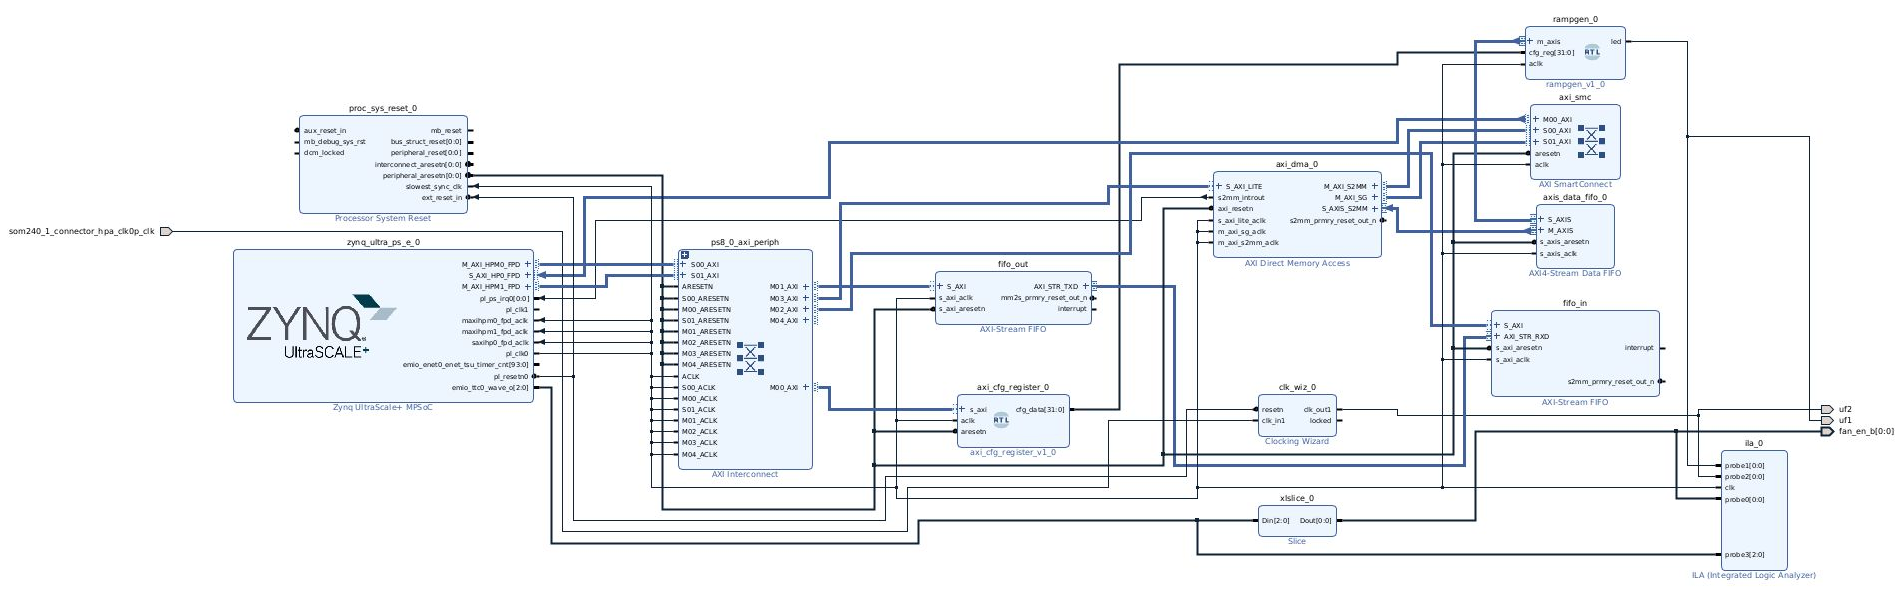
\includegraphics[width=1\textwidth]{images/dma}
	\caption{Vivado DMA block scheme.}
	\label{fig:dma}
\end{figure}
The block scheme is composed by the following blocks:
\begin{itemize}
	\item Zynq UltraScale+ Processing System: This is a highly versatile and powerful System-on-Chip (SoC) that combines programmable logic (FPGA fabric) and processing capabilities (ARM Cortex cores). It's the brain of the system, handling computation, decision-making, and coordination between other components.
	
	\item AXI Direct Memory Access (DMA): This block facilitates high-speed data transfer between memory and peripherals or other components, bypassing the CPU. It’s crucial for efficient data handling in high-performance systems.
	
	\item FIFO (First-In, First-Out): A type of data buffer used to ensure smooth and orderly data flow. It stores data temporarily and releases it in the same order it was received, preventing bottlenecks in the system.
	
	\item AXI Interconnect: This connects various AXI-based components within the design. It manages data flow between the processor, peripherals, memory, and other AXI-compatible blocks, ensuring efficient communication.
	
	\item Peripheral Interfaces: These are bridges connecting external devices (like sensors, displays, or communication modules) to the main system. They ensure compatibility and proper data exchange between the system and peripherals.
	
	\item Memory Controller: This manages the read and write operations to and from external or on-chip memory, ensuring data is stored and accessed efficiently.
\end{itemize}



\section{Petalinux project}
Despite having created the Vivado project and established a design flow, the current approach does not work in this case. The previous method was discovered through trial and error rather than a structured research effort like this one. The main issue arises during board boot: the DMA controller attempts to access memory addresses defined in the Vivado block design before the FPGA has been programmed. To address this, the device tree is modified after boot, creating a custom configuration to ensure proper memory access and system functionality. To upload the code relative to the DMA testing, there are few steps to follow:
\begin{itemize}
	\item The first step is to create the file \textbf{pl-<projectname>.dtsi}. The file has to be modified as shown in the following code. The node \textit{fragment@1} is copied from \textbf{pl.dtsi} (found in \textit{components/plnx\_workspace/device-tree/device-tree/}. In addition all the data relative to the DMA and the memory instantiation are copied. \textbf{dmatest\_0} has to be written anew instead, since it is not found in any file.
	\vspace{0.1cm}
	\begin{lstlisting}[language=C]
		/*
		* CAUTION: This file is automatically generated by Xilinx.
		* Version: XSCT
		* Today is: Wed Feb 26 13:53:04 2025
		*/
		
		
		/dts-v1/;
		/plugin/;
		/ {
			fragment@1 {
				target = <&amba>;
				overlay1: __overlay__ {
					#address-cells = <2>;
					#size-cells = <2>;
					afi0: afi0 {
						compatible = "xlnx,afi-fpga";
						config-afi = < 0 2>, <1 2>, <2 0>, <3 0>, <4 2>, <5 2>, <6 0>, <7 0>, <8 0>, <9 0>, <10 0>, <11 0>, <12 0>, <13 0>, <14 0xa00>, <15 0x000>;
					};
					clocking0: clocking0 {
						#clock-cells = <0>;
						assigned-clock-rates = <99999001>;
						assigned-clocks = <&zynqmp_clk 71>;
						clock-output-names = "fabric_clk";
						clocks = <&zynqmp_clk 71>;
						compatible = "xlnx,fclk";
					};
					clocking1: clocking1 {
						#clock-cells = <0>;
						assigned-clock-rates = <99999001>;
						assigned-clocks = <&zynqmp_clk 72>;
						clock-output-names = "fabric_clk";
						clocks = <&zynqmp_clk 72>;
						compatible = "xlnx,fclk";
					};
					
					dmatest_0: dmatest@0 {
						compatible ="xlnx,axi-dma-test-1.00.a";
						dmas = <&axi_dma_0 1>;
						dma-names = "dma0";
					};
					axi_cfg_register_0: axi_cfg_register@b0000000 {
						clock-names = "aclk";
						clocks = <&zynqmp_clk 71>;
						compatible = "xlnx,axi-cfg-register-1.0";
						reg = <0x0 0xb0000000 0x0 0x80>;
					};
					axi_dma_0: dma@a0020000 {
						#dma-cells = <1>;
						clock-names = "m_axi_s2mm_aclk", "m_axi_sg_aclk", "s_axi_lite_aclk";
						clocks = <&zynqmp_clk 71>, <&zynqmp_clk 71>, <&zynqmp_clk 71>;
						compatible = "xlnx,axi-dma-7.1", "xlnx,axi-dma-1.00.a";
						interrupt-names = "s2mm_introut";
						interrupt-parent = <&gic>;
						interrupts = <0 89 4>;
						reg = <0x0 0xa0020000 0x0 0x10000>;
						xlnx,addrwidth = <0x20>;
						xlnx,include-sg ;
						xlnx,sg-length-width = <0x17>;
						dma-channel@a0020030 {
							compatible = "xlnx,axi-dma-s2mm-channel";
							dma-channels = <0x1>;
							interrupts = <0 89 4>;
							xlnx,datawidth = <0x20>;
							xlnx,device-id = <0x0>;
						};
					};
					fifo_in: axi_fifo_mm_s@a0010000 {
						clock-names = "s_axi_aclk";
						clocks = <&zynqmp_clk 71>;
						compatible = "xlnx,axi-fifo-mm-s-4.3";
						reg = <0x0 0xa0010000 0x0 0x10000>;
						xlnx,axi-str-rxd-protocol = "XIL_AXI_STREAM_ETH_DATA";
						xlnx,axi-str-rxd-tdata-width = <0x20>;
						xlnx,axi-str-txc-protocol = "XIL_AXI_STREAM_ETH_CTRL";
						xlnx,axi-str-txc-tdata-width = <0x20>;
						xlnx,axi-str-txd-protocol = "XIL_AXI_STREAM_ETH_DATA";
						xlnx,axi-str-txd-tdata-width = <0x20>;
						xlnx,axis-tdest-width = <0x4>;
						xlnx,axis-tid-width = <0x4>;
						xlnx,axis-tuser-width = <0x4>;
						xlnx,data-interface-type = <0x0>;
						xlnx,has-axis-tdest = <0x0>;
						xlnx,has-axis-tid = <0x0>;
						xlnx,has-axis-tkeep = <0x0>;
						xlnx,has-axis-tstrb = <0x0>;
						xlnx,has-axis-tuser = <0x0>;
						xlnx,rx-cascade-height = <0x0>;
						xlnx,rx-enable-ecc = <0x0>;
						xlnx,rx-fifo-depth = <0x800>;
						xlnx,rx-fifo-pe-threshold = <0x5>;
						xlnx,rx-fifo-pf-threshold = <0x1fb>;
						xlnx,rx-has-ecc-err-inject = <0x0>;
						xlnx,s-axi-id-width = <0x4>;
						xlnx,s-axi4-data-width = <0x20>;
						xlnx,select-xpm = <0x0>;
						xlnx,tx-cascade-height = <0x0>;
						xlnx,tx-enable-ecc = <0x0>;
						xlnx,tx-fifo-depth = <0x200>;
						xlnx,tx-fifo-pe-threshold = <0x5>;
						xlnx,tx-fifo-pf-threshold = <0x1fb>;
						xlnx,tx-has-ecc-err-inject = <0x0>;
						xlnx,use-rx-cut-through = <0x0>;
						xlnx,use-rx-data = <0x1>;
						xlnx,use-tx-ctrl = <0x0>;
						xlnx,use-tx-cut-through = <0x0>;
						xlnx,use-tx-data = <0x0>;
					};
					fifo_out: axi_fifo_mm_s@a0000000 {
						clock-names = "s_axi_aclk";
						clocks = <&zynqmp_clk 71>;
						compatible = "xlnx,axi-fifo-mm-s-4.3";
						reg = <0x0 0xa0000000 0x0 0x10000>;
						xlnx,axi-str-rxd-protocol = "XIL_AXI_STREAM_ETH_DATA";
						xlnx,axi-str-rxd-tdata-width = <0x20>;
						xlnx,axi-str-txc-protocol = "XIL_AXI_STREAM_ETH_CTRL";
						xlnx,axi-str-txc-tdata-width = <0x20>;
						xlnx,axi-str-txd-protocol = "XIL_AXI_STREAM_ETH_DATA";
						xlnx,axi-str-txd-tdata-width = <0x20>;
						xlnx,axis-tdest-width = <0x4>;
						xlnx,axis-tid-width = <0x4>;
						xlnx,axis-tuser-width = <0x4>;
						xlnx,data-interface-type = <0x0>;
						xlnx,has-axis-tdest = <0x0>;
						xlnx,has-axis-tid = <0x0>;
						xlnx,has-axis-tkeep = <0x0>;
						xlnx,has-axis-tstrb = <0x0>;
						xlnx,has-axis-tuser = <0x0>;
						xlnx,rx-cascade-height = <0x0>;
						xlnx,rx-enable-ecc = <0x0>;
						xlnx,rx-fifo-depth = <0x200>;
						xlnx,rx-fifo-pe-threshold = <0x5>;
						xlnx,rx-fifo-pf-threshold = <0x1fb>;
						xlnx,rx-has-ecc-err-inject = <0x0>;
						xlnx,s-axi-id-width = <0x4>;
						xlnx,s-axi4-data-width = <0x20>;
						xlnx,select-xpm = <0x0>;
						xlnx,tx-cascade-height = <0x0>;
						xlnx,tx-enable-ecc = <0x0>;
						xlnx,tx-fifo-depth = <0x800>;
						xlnx,tx-fifo-pe-threshold = <0x5>;
						xlnx,tx-fifo-pf-threshold = <0x1fb>;
						xlnx,tx-has-ecc-err-inject = <0x0>;
						xlnx,use-rx-cut-through = <0x0>;
						xlnx,use-rx-data = <0x0>;
						xlnx,use-tx-ctrl = <0x0>;
						xlnx,use-tx-cut-through = <0x1>;
						xlnx,use-tx-data = <0x1>;
					};
					
				};
			};
		};
	\end{lstlisting}
	\vspace{0.1cm}
	\item The second step is to compile the file just created. Move into the folder \textit{project-name/build/tmp/sysroots-components/x86\_64/dtc-native/usr/bin/} and with the command
	\vspace{0.1cm}
	\begin{lstlisting}[language=bash]
		dtc -@  -I dts -O dtb -o pl-gabriele.dtbo pl-gabriele.dtsi
	\end{lstlisting}
	compile the new device tree. This latter command creates the .dtbo file for the device tree just created.
	
	\item The last step is to copy all the necessary files into the bard, to program the FPGA and to load the new device tree. All this steps can be executed with the following commands
		\vspace{0.1cm}
	\begin{lstlisting}[language=bash]
	sudo cp pl-gabriele.dtbo design_1_wrapper.bin /lib/firmware/
	sh -c 'echo "design_1_wrapper.bin" > /sys/class/fpga_manager/fpga0/firmware'
	mkdir /sys/kernel/config/device-tree/overlays/pl-gabriele
	sh -c  'echo "pl-gabriele.dtbo" > /sys/kernel/config/device-tree/overlays/pl-gabriele/path'
	\end{lstlisting}
	\vspace{0.1cm}
\end{itemize}



\subsection{Driver deployment}
After having successfully build the new additional device tree, performing read/write operations on the memories and registers requires the definition of two additional components: a) the Driver, responsible for managing communication between the PS and the PL and b) the user program, which executes the operations using the driver to interact with the hardware. The driver must then be compiled into a .ko (Kernel Object) file, which can be loaded and executed on the KRIA board. The procedure to achieve this is quite complex, and even small mistakes can lead to errors. Therefore, careful attention is required at each step to ensure successful implementation.

An automatic Python-based generator is used to create the driver, which takes as input: a) the name of the driver b) the path to system-user.dtsi and c) the name of an input FIFO (only if read direct read operation are needed, in the case of the DMA there it is not requested). The generator produces the driver's template files (.c and .h). The steps to correctly define deploy the driver are the following:
\begin{enumerate}
	\item Create the driver module using the command
	\vspace{0.1cm}
	\begin{lstlisting}[language=bash]
		petalinux-create -t modules --name driver_name --enable	\end{lstlisting}
		
	\item Copy the template files into \textit{project-spec/meta-user/recipes-modules/driver\_name/files/}.
	
	\item Modify the Makefile to include the path to the .h file in the \textbf{MY\_CFLAGS} line. Not including the path will result in an error, as PetaLinux will be unable to locate such file. The updated Makefile is shown below:
	\vspace{0.1cm}
	\begin{lstlisting}[language=make]
		obj-m := blinkdriver.o
		
		MY_CFLAGS += -g -DDEBUG -I /data/devel/kria_mb/ptlnx/prj/blink_mk_VIII/project-spec/meta-user/recipes-modules/blinkdriver/files
		ccflags-y += ${MY_CFLAGS}
		
		SRC := $(shell pwd)
		
		all:
		$(MAKE) -C $(KERNEL_SRC) M=$(SRC)
		
		modules_install:
		$(MAKE) -C $(KERNEL_SRC) M=$(SRC) modules_install
		
		clean:
		rm -f *.o *~ core .depend .*.cmd *.ko *.mod.c
		rm -f Module.markers Module.symvers modules.order
		rm -rf .tmp_versions Modules.symvers
	\end{lstlisting}
	
	Build the driver using
	\vspace{0.1cm}
	\begin{lstlisting}[language=bash]
		petalinux-build -c driver_name	\end{lstlisting}
		
	\item Locate the .ko file and copy it, through ssh, to the KRIA along with the .h file. Move also the .bin file.
	
	\item Program the FPGA (see previous chapter).
	
	\item With the command 
	\vspace{0.1cm}
	\begin{lstlisting}[language=bash]
		sudo insmod driver_name.ko	\end{lstlisting}
	launch the driver in the KRIA. 
	
	\item This last step has to be done after the program that will make use of the driver has been written and complied. Once the program is done then type
	\vspace{0.1cm}
	\begin{lstlisting}[language=bash]
		./program_name	\end{lstlisting}
	and now everything should be working properly.
\end{enumerate}

	
\end{document}